\chapter{Logiche Temporali Ramificate e Model Checking a Punto Fisso}\label{ch:ctl}

Passiamo ora dalle logiche temporali lineari a quelle \keyword{ramificate}, in particolare con \(CTL^*\) (\textit{full computation tree logic}), che contiene LTL ma permette di esprimere anche proprietà su come le computazioni si diramano, non esprimibili in LTL\@.

Studieremo in particolare il frammento \(CTL\), un sottoinsieme di \(CTL^*\) più facile da verificare, di cui vorremo risolvere il model checking. Vedremo inizialmente un algoritmo diretto per il model checking di \(CTL\) basato sull'etichettatura degli stati, poi la sua rilettura in termini di teoria dei punti fissi, che sarà la base per l'algoritmo simbolico più efficiente basato sugli OBDD del prossimo capitolo.

\section{La logica \texorpdfstring{\(CTL^*\)}{CTL*}}

L'idea centrale è aggiungere dei \keyword{quantificatori sui percorsi}, \(A\) ed \(E\), che indicano rispettivamente che una proprietà di percorso è vera su \emph{tutti} i percorsi o su \emph{almeno uno} dei percorsi uscenti da uno stato.

\begin{definition}{Grammatica di \(CTL^*\)}
  La grammatica di \(CTL^*\) è formata da due grammatiche mutuamente ricorsive, quella delle \keyword{formule di stato} \(\phi\) e quella delle \keyword{formule di percorso} \(\psi\):
  \[\phi ::= p \in AP \mid \neg \phi \mid \phi \land \phi \mid \phi \lor \phi \mid A\psi \mid E\psi\]
  \[\psi ::= \phi \mid \neg \psi \mid \psi \land \psi \mid \psi \lor \psi \mid X\psi \mid \psi U\psi \mid \psi R\psi\]
\end{definition}

Possiamo vedere \(\psi\) come LTL \q{sopra} le formule di stato \(\phi\). 

Per quanto riguarda la semantica invece, per la sua natura ramificata, non è più sufficiente avere come modello una stringa (finita o infinita che sia), ma sarà necessario da subito considerare l'intera struttura di Kripke, che prima fungeva solo da \qi{generatore} di modelli.

In un certo senso ci si è spostati in alto di un livello, considerando nel linguaggio oggetto quello che prima era parte del meta-linguaggio.

Anche per \(LTL\) infatti si era esteso il concetto di soddisfazione di una formula da parte di una struttura di Kripke, dandone però semantica solo al meta-livello, nella definizione della relazione di soddisfazione, e mai nella semantica della logica stessa.

In LTL avevamo infatti che \(K \models_{LTL} \psi\) se ogni percorso della struttura di Kripke soddisfa la formula. Ora possiamo esprimere la stessa cosa in \(CTL^*\) come \(K \models_{CTL^*} A\psi\).

Vediamo quindi in tutti i dettagli come dare semantica al linguaggio di \(CTL^*\).

\begin{definition}{Semantica di \(CTL^*\)}
  Data una struttura di Kripke \(K = \langle AP, W, R, w_0, \lambda \rangle\) e uno stato \(w \in W\) (se omesso, \(w_0\)), la semantica delle formule di stato è:
  \begin{itemize}
    \item \(K,w \models p\) se e solo se \(p \in \lambda(w)\)
    \item \(K,w \models \neg \phi\) se e solo se \(K,w \not\models \phi\)
    \item \(K,w \models \phi_1 \land \phi_2\) se e solo se \(K,w \models \phi_1\) e \(K,w \models \phi_2\)
    \item \(K,w \models \phi_1 \lor \phi_2\) se e solo se \(K,w \models \phi_1\) o \(K,w \models \phi_2\)
    \item \(K,w \models A\psi\) se e solo se \(\forall \pi \in Paths(K,w),\ K,\pi \models \psi\)
    \item \(K,w \models E\psi\) se e solo se \(\exists \pi \in Paths(K,w),\ K,\pi \models \psi\)
  \end{itemize}
  La semantica delle formule di percorso \(\psi\) è esattamente quella di LTL, con l'unica differenza del caso base, generalizzato da \(p\) a \(\phi\):
  \[K, \pi, i\models \phi \text{ se e solo se } K,{(\pi)}_i\models \phi\]
\end{definition}

\begin{note}{}
  Fino ai quantificatori sui percorsi la semantica è definita su \emph{stati}, e non ha alcuna nozione temporale; nei quantificatori si passa alla semantica LTL, definita sui \emph{percorsi}. A LTL basterebbe il percorso \(\pi\), ma poiché in una formula di percorso si può tornare a una formula di stato, è necessario mantenere anche la struttura \(K\) per poter valutare le formule di stato annidate.
\end{note}

\section{Il frammento \(CTL\)}

\keyword{CTL} è il sottoinsieme di \(CTL^*\) in cui ogni operatore temporale è \emph{immediatamente} preceduto da un quantificatore sui percorsi. Ciò che cambia è la grammatica delle formule di percorso, che si riduce a:
\[\psi ::= X\phi \mid \phi U\phi \mid \phi R\phi\]

In questo modo non c'è nesting libero di operatori temporali. Una formulazione alternativa, e storicamente la prima proposta, usa un'unica grammatica con operatori composti:
\[\phi ::= p \in AP \mid \neg \phi \mid \phi \land \phi \mid \phi \lor \phi \mid AX\phi \mid EX\phi \mid A(\phi U \phi) \mid A(\phi R \phi) \mid E(\phi U \phi) \mid E(\phi R \phi)\]

Questa sintassi esplicita è più prolissa, ma è usata in molti software perché il model checking di \(CTL\) si risolve proprio per sottoproblemi sulle sottoformule di questa forma, combinandone poi i risultati.

\subsection{Il frammento esistenziale}

Come di consueto, conviene individuare un insieme minimale di operatori, eliminando quelli esprimibili tramite dualità. Oltre alle solite dualità booleane, ogni coppia di operatori duali permette un'eliminazione:
\[\neg AX\phi \equiv E\neg X \phi \equiv EX \neg \phi\]
quindi \(AX\) è ridondante. Similmente
\[\neg A (\phi_1 U \phi_2) \equiv E \neg (\phi_1 U \phi_2) \equiv E (\neg \phi_1 R \neg \phi_2)\]
e di conseguenza \(AU\), e analogamente \(AR\), sono ridondanti. A livello algoritmico è dunque sufficiente considerare il \keyword{frammento esistenziale} di \(CTL\), che contiene solo \(E\) come quantificatore.

Possiamo ridurre ulteriormente gli operatori osservando la semantica del release: se \(\phi_1\) non è mai vera, allora \(\phi_1 R \phi_2\) è vera se e solo se \(\phi_2\) è sempre vera, ovvero \(G\phi_2\); altrimenti \(\phi_2\) dev'essere vera fino a quando (compreso) \(\phi_1\) diventa vera. Formalmente, dalla semantica
\[\pi, i \models \phi_1 R \phi_2 \iff \forall j \geq i.\ \left(\pi, j \models \phi_2 \lor \exists k\st i \leq k < j \land \pi, k \models \phi_1 \land \phi_2\right)\]
si ottiene l'equivalenza \(\phi_1 R \phi_2 \equiv G \phi_2 \lor (\phi_2 U (\phi_1 \land \phi_2))\). A livello di \(CTL\), essendo che \(E\) distribuisce su \(\lor\), abbiamo
\[E (\phi_1 R \phi_2) \equiv E G\phi_2 \lor E (\phi_2 U(\phi_1 \land \phi_2))\]

Dunque la logica che andremo effettivamente a risolvere è la seguente:
\[\phi::= p \in AP \mid \neg \phi \mid \phi \lor \phi \mid EX \phi \mid E(\phi U \phi) \mid EG \phi\]

\subsection{One-step unfolding in \(CTL\)}

Per gli algoritmi ci serve estendere a \(CTL\) la proprietà di one-step unfolding vista per LTL\@. Partendo da \(\phi_1 U \phi_2 \equiv \phi_2 \lor (\phi_1 \land X(\phi_1 U \phi_2))\), in \(CTL^*\) abbiamo:
\[E(\phi_1 U \phi_2 )\equiv E(\phi_2 \lor (\phi_1 \land X(\phi_1 U \phi_2))) \equiv E\phi_2 \lor E(\phi_1 \land X(\phi_1 U \phi_2))\]

Nella sintassi di \(CTL\) non possiamo scrivere \(E \phi_2\) con \(\phi_2\) formula di stato, ma ciò che questa formula chiede è che esista un percorso il cui primo stato soddisfa \(\phi_2\): equivale a richiedere semplicemente \(\phi_2\). Per quanto riguarda \(E(\phi_1 \land X(\phi_1 U \phi_2))\), stiamo richiedendo che esista un percorso in cui \(\phi_1\) è vera in radice e il cui suffisso dal secondo stato soddisfa \(\phi_1 U \phi_2\): equivale a \(\phi_1 \land EX (E (\phi_1 U \phi_2))\). Otteniamo dunque il one-step unfolding in \(CTL\):
\[E(\phi_1 U \phi_2) \equiv \phi_2 \lor (\phi_1 \land EX (E (\phi_1 U \phi_2)))\]

Per \(EG\) passiamo per il release: da
\[E(\phi_1 R \phi_2) \equiv E(\phi_2 \land (\phi_1 \lor X(\phi_1 R \phi_2))) \equiv \phi_2 \land (\phi_1 \lor EX (E (\phi_1 R \phi_2)))\]
ed essendo \(G \phi_2 \equiv \bot R \phi_2\), sostituendo e semplificando \(\bot\):
\[EG \phi \equiv \phi \land EX (EG \phi)\]

\section{Model checking di \(CTL\) per etichettatura}

L'algoritmo di model checking di \(CTL\) procede \keyword{bottom-up}: si risolvono prima le sottoformule più interne e si etichetta ogni stato del modello con le formule che vi sono soddisfatte, risalendo fino alla formula \(\phi\) da verificare. Alla fine, \(K \models \phi\) se e solo se lo stato iniziale è etichettato con \(\phi\).

Formalizziamo prima l'insieme delle sottoformule rilevanti, in analogia con la chiusura vista per LTL, per il frammento esistenziale:

\begin{definition}{Chiusura di una formula \(CTL\)}
  \(cl(\phi)\) è il più piccolo insieme tale che:
  \begin{itemize}
    \item \(\phi \in cl(\phi)\)
    \item \(\neg \phi' \in cl(\phi)\implies \phi' \in cl(\phi)\)
    \item \(\phi_1 \lor \phi_2 \in cl(\phi)\implies \phi_1, \phi_2 \in cl(\phi)\)
    \item \(EX \phi' \in cl(\phi)\implies \phi' \in cl(\phi)\)
    \item \(E(\phi_1 U \phi_2) \in cl(\phi)\implies \phi_1, \phi_2 \in cl(\phi)\)
    \item \(EG \phi' \in cl(\phi)\implies \phi' \in cl(\phi)\)
  \end{itemize}
\end{definition}

L'algoritmo etichetta ogni stato con le formule di \(cl(\phi)\) soddisfatte in quello stato, partendo dalle proposizioni atomiche. I casi booleani sono immediati; vediamo i tre operatori temporali.\footnote{Il tipo \(Unit\) rappresenta l'assenza di un valore di ritorno: le funzioni vengono eseguite per il loro effetto collaterale di aggiornare l'etichettatura \(\lambda\).}

\subsection{Checking di \texorpdfstring{\(EX\)}{EX}}

Per \(EX\phi\) è sufficiente etichettare tutti i predecessori degli stati che soddisfano \(\phi\):

\begin{algorithmdesc}{Checking \(EX\)}
  \begin{algorithmic}[1]
    \Statex{} \textbf{signature} \(\textsc{CheckEX:} \quad Kripke \times Formula \to Unit\)
    \Function{\(\textsc{CheckEX}\)}{$(K,\phi)$} % chktex 46
    \State{} \(T \gets \set{w \in W}[\phi \in \lambda(w)]\)
    \While{\(T\neq \emptyset\)}
    \State{} \(s \gets\) choose \(T\)
    \State{} \(T \gets T\setminus\set{s}\)
    \For{\(t \in R^{-1}(s)\)}
    \State{} \(\lambda(t)\gets \lambda(t)\cup\set{EX \phi}\)
    \EndFor{}
    \EndWhile{}
    \EndFunction{}
  \end{algorithmic}
\end{algorithmdesc}

\subsection{Checking di \texorpdfstring{\(EU\)}{EU}}

Per \(E(\phi_1 U \phi_2)\) sfruttiamo il one-step unfolding \(E (\phi_1 U \phi_2) \equiv \phi_2 \lor (\phi_1 \land EX(E (\phi_1 U \phi_2)))\): partiamo dagli stati che soddisfano \(\phi_2\), che sicuramente soddisfano \(E(\phi_1 U \phi_2)\), e procediamo a ritroso, poiché gli stati entranti in stati che soddisfano \(E (\phi_1 U \phi_2)\) soddisfano \(EX(E (\phi_1 U \phi_2))\): basterà controllare che soddisfino anche \(\phi_1\) per avere l'altro disgiunto.

Consideriamo la formula \(E(p\,U\,q)\) e la struttura di Kripke seguente. Lo stato \(s_2\) soddisfa \(q\), mentre \(s_0\) e \(s_1\) soddisfano \(p\). Il self-loop su \(s_2\) rende esplicito che da lì è possibile proseguire indefinitamente.

\begin{figure}[H]
  \centering
  \begin{tikzpicture}[shorten >=1pt,node distance=1.55cm,on grid,auto,font=\small]
    \begin{scope}
      \node[state] (eu_s0)                      {\(s_0\)};
      \node[state] (eu_s1) [right=of eu_s0]     {\(s_1\)};
      \node[state,accepting] (eu_s2) [right=of eu_s1]     {\(s_2\)};
      \path[->]
        (eu_s0) edge node {\(\)} (eu_s1)
        (eu_s1) edge node {\(\)} (eu_s2)
        (eu_s2) edge [loop above] node {\(\)} ();
      \node[below=0.35cm of eu_s0] {\(p\)};
      \node[below=0.35cm of eu_s1] {\(p\)};
      \node[below=0.35cm of eu_s2] {\(q\)};
      \node[below=1.05cm of eu_s1] {Struttura di Kripke};
    \end{scope}

    \begin{scope}[xshift=4.35cm]
      \node[state] (eu_i0)                      {\(s_0\)};
      \node[state,accepting] (eu_i1) [right=of eu_i0]     {\(s_1\)};
      \node[state,accepting] (eu_i2) [right=of eu_i1]     {\(s_2\)};
      \path[->]
        (eu_i0) edge node {\(\)} (eu_i1)
        (eu_i1) edge node {\(\)} (eu_i2)
        (eu_i2) edge [loop above] node {\(\)} ();
      \node[below=0.35cm of eu_i0] {\(p\)};
      \node[below=0.35cm of eu_i1] {\(p\)};
      \node[below=0.35cm of eu_i2] {\(q\)};
      \node[below=1.05cm of eu_i1] {Inizializzazione: \(\den{q}\)};
    \end{scope}

    \begin{scope}[xshift=8.7cm]
      \node[state,accepting] (eu_f0)                      {\(s_0\)};
      \node[state,accepting] (eu_f1) [right=of eu_f0]     {\(s_1\)};
      \node[state,accepting] (eu_f2) [right=of eu_f1]     {\(s_2\)};
      \path[->]
        (eu_f0) edge node {\(\)} (eu_f1)
        (eu_f1) edge node {\(\)} (eu_f2)
        (eu_f2) edge [loop above] node {\(\)} ();
      \node[below=0.35cm of eu_f0] {\(p\)};
      \node[below=0.35cm of eu_f1] {\(p\)};
      \node[below=0.35cm of eu_f2] {\(q\)};
      \node[below=1.05cm of eu_f1] {Punto fisso: \(\den{E(p\,U\,q)}\)};
    \end{scope}
  \end{tikzpicture}
  \caption{Evoluzione dell'etichettatura per il checking di \(E(p\,U\,q)\).}
  \label{fig:ctl-eu-labeling}
\end{figure}

Più precisamente, l'immagine mostra tre istanti dell'algoritmo. Inizialmente si etichetta \(s_2\), perché soddisfa \(q\). Poiché \(s_1\) soddisfa \(p\) e ha un successore già etichettato, si aggiunge \(s_1\); nella passata successiva lo stesso ragionamento aggiunge \(s_0\). Si raggiunge quindi il punto fisso
\[
  \den{E(p\,U\,q)}=\{s_0,s_1,s_2\}.
\]
Il percorso \(s_0s_1s_2s_2\ldots\) è infatti un testimone della formula: prima di raggiungere \(q\), tutti gli stati soddisfano \(p\).

\begin{algorithmdesc}{Checking \(EU\)}
  \begin{algorithmic}[1]
    \Statex{} \textbf{signature} \(\textsc{CheckEU:} \quad Kripke \times Formula \times Formula \to Unit\)
    \Function{\(\textsc{CheckEU}\)}{$(K,\phi_1,\phi_2)$} % chktex 46
    \State{} \(T \gets \set{w \in W}[ \phi_2 \in \lambda(w)]\)
    \For{\(w \in T\)}
    \State{} \(\lambda(w) \gets \lambda(w)\cup\set{E (\phi_1 U \phi_2)}\)
    \EndFor{}
    \While{\(T\neq \emptyset\)}
    \State{} \(s \gets\) choose \(T\)
    \State{} \(T \gets T\setminus\set{s}\)
    \For{\(t \in R^{-1}(s)\)}
    \If{\(E(\phi_1 U \phi_2) \notin \lambda(t) \land \phi_1 \in \lambda(t)\)}
    \State{} \(\lambda(t) \gets \lambda(t)\cup\set{E (\phi_1 U \phi_2)}\)
    \State{} \(T \gets T\cup\set{t}\)
    \EndIf{}
    \EndFor{}
    \EndWhile{}
    \EndFunction{}
  \end{algorithmic}
\end{algorithmdesc}

La complessità è chiaramente lineare nelle dimensioni del grafo, ovvero \(\BigO{\abs{W} + \abs{R}}\) per una struttura di Kripke.

\subsection{Checking di \texorpdfstring{\(EG\)}{EG}}

Per \(EG\phi\), sfruttando \(EG \phi \equiv \phi \land EX (EG \phi)\), il modo più semplice è calcolare le componenti fortemente connesse (SCC) del sottografo formato dagli stati che soddisfano \(\phi\): gli stati delle SCC non banali soddisfano \(EG \phi\) (vi si può ciclare per sempre rimanendo in stati che soddisfano \(\phi\)), e poi si procede a ritroso per etichettare anche gli stati che raggiungono tali componenti passando solo per stati che soddisfano \(\phi\).

Consideriamo la formula \(EGp\) e la struttura di Kripke seguente. Tutti gli stati soddisfano \(p\); lo stato \(s_2\) appartiene a una SCC non banale grazie al self-loop, e può quindi essere visitato indefinitamente. Gli stati \(s_1\) e \(s_0\) vengono poi etichettati propagando all'indietro lungo il cammino che conduce a \(s_2\).

\begin{figure}[H]
  \centering
  \begin{tikzpicture}[shorten >=1pt,node distance=1.55cm,on grid,auto,font=\small]
    \begin{scope}
      \node[state] (eg_s0)                  {\(s_0\)};
      \node[state] (eg_s1) [right=of eg_s0] {\(s_1\)};
      \node[state] (eg_s2) [right=of eg_s1] {\(s_2\)};
      \path[->]
        (eg_s0) edge (eg_s1)
        (eg_s1) edge (eg_s2)
        (eg_s2) edge [loop above] ();
      \node[below=0.35cm of eg_s0] {\(p\)};
      \node[below=0.35cm of eg_s1] {\(p\)};
      \node[below=0.35cm of eg_s2] {\(p\)};
      \node[below=1.05cm of eg_s1] {Struttura di Kripke};
    \end{scope}

    \begin{scope}[xshift=4.35cm]
      \node[state] (eg_i0)                  {\(s_0\)};
      \node[state] (eg_i1) [right=of eg_i0] {\(s_1\)};
      \node[state,accepting] (eg_i2) [right=of eg_i1] {\(s_2\)};
      \path[->]
        (eg_i0) edge (eg_i1)
        (eg_i1) edge (eg_i2)
        (eg_i2) edge [loop above] ();
      \node[below=0.35cm of eg_i0] {\(p\)};
      \node[below=0.35cm of eg_i1] {\(p\)};
      \node[below=0.35cm of eg_i2] {\(p\)};
      \node[below=1.05cm of eg_i1] {Inizializzazione: SCC non banale};
    \end{scope}

    \begin{scope}[xshift=8.7cm]
      \node[state,accepting] (eg_f0)                  {\(s_0\)};
      \node[state,accepting] (eg_f1) [right=of eg_f0] {\(s_1\)};
      \node[state,accepting] (eg_f2) [right=of eg_f1] {\(s_2\)};
      \path[->]
        (eg_f0) edge (eg_f1)
        (eg_f1) edge (eg_f2)
        (eg_f2) edge [loop above] ();
      \node[below=0.35cm of eg_f0] {\(p\)};
      \node[below=0.35cm of eg_f1] {\(p\)};
      \node[below=0.35cm of eg_f2] {\(p\)};
      \node[below=1.05cm of eg_f1] {Punto fisso: \(\den{EGp}\)};
    \end{scope}
  \end{tikzpicture}
  \caption{Evoluzione dell'etichettatura per il checking di \(EGp\).}\label{fig:ctl-eg-labeling}
\end{figure}

Più precisamente, l'algoritmo individua inizialmente \(s_2\), che appartiene a una SCC con un ciclo. Da \(s_2\) si può quindi costruire un percorso infinito che rimane in stati che soddisfano \(p\), perciò \(s_2\models EGp\). Poiché \(s_1\) ha un successore già etichettato con \(EGp\) e soddisfa \(p\), viene etichettato a sua volta; lo stesso vale poi per \(s_0\). Al punto fisso si ottiene
\[
  \den{EGp}=\{s_0,s_1,s_2\}.
\]
Il percorso \(s_0s_1s_2s_2\ldots\) è infatti un testimone della formula: da ogni stato è possibile proseguire scegliendo un successore e mantenendo sempre vera \(p\).

\begin{algorithmdesc}{Checking \(EG\)}
  \begin{algorithmic}[1]
    \Statex{} \textbf{signature} \(\textsc{CheckEG:} \quad Kripke \times Formula \to Unit\)
    \Function{\(\textsc{CheckEG}\)}{$(K,\phi)$} % chktex 46
    \State{} \(S \gets \set{w \in W}[\phi \in \lambda(w)]\)
    \State{} \(G \gets (S, R\cap(S\times S))\)
    \State{} \(SCC^* \gets \set{C \in SCC(G)}[\abs{C} + \abs{R\cap(C\times C)} > 1]\)
    \State{} \(T \gets \bigcup SCC^*\)
    \For{\(w \in T\)}
    \State{} \(\lambda(w) \gets \lambda(w)\cup\set{E G \phi}\)
    \EndFor{}
    \While{\(T\neq \emptyset\)}
    \State{} \(s \gets\) choose \(T\)
    \State{} \(T \gets T\setminus\set{s}\)
    \For{\(t \in R^{-1}(s)\)}
    \If{\(EG\phi \notin \lambda(t) \land \phi \in \lambda(t)\)}
    \State{} \(\lambda(t) \gets \lambda(t)\cup\set{E G \phi}\)
    \State{} \(T \gets T\cup\set{t}\)
    \EndIf{}
    \EndFor{}
    \EndWhile{}
    \EndFunction{}
  \end{algorithmic}
\end{algorithmdesc}

Anche in questo caso la complessità è lineare, poiché il calcolo delle SCC (ad esempio con l'algoritmo di Tarjan) è lineare. Complessivamente, il model checking di \(CTL\) costa \(\BigO{\abs{\phi}\cdot(\abs{W} + \abs{R})}\), poiché ogni sottoformula richiede una passata lineare.

\section{Teoria dei punti fissi}

Gli algoritmi appena visti hanno una struttura comune: partono da un insieme di stati e lo estendono (o restringono) iterativamente fino a stabilizzarsi. Questa struttura non è casuale: è un'istanza del calcolo di \keyword{punti fissi} di funzioni monotone, che formalizziamo ora. Questa rilettura sarà essenziale per il model checking simbolico.

Data una funzione \(f\), un \keyword{punto fisso} è un elemento \(x\) tale che \(f(x) = x\). Nel nostro contesto le funzioni assoceranno insiemi di stati a insiemi di stati: per \(U\) partiremo da un insieme minimo di stati che soddisfano la formula e iterativamente ne aggiungeremo fino a raggiungere il \emph{minimo} punto fisso; dualmente per \(G\) partiremo da tutti gli stati e ne toglieremo fino al \emph{massimo} punto fisso.

\subsection{Ordini parziali e monotonia}

\begin{definition}{Ordine parziale, estremi, catene}
  Consideriamo una struttura d'ordine parziale \(\mathcal{P} = \langle P, \sqsubseteq \rangle\), con \(P\) insieme e \(\sqsubseteq\) relazione d'ordine parziale su \(P\). Dato \(P'\subseteq P\):
  \begin{itemize}
    \item \(p\) è un \keyword{maggiorante} di \(P'\) se \(\forall p' \in P',\ p' \sqsubseteq p\); dualmente \(p\) è un \keyword{minorante} di \(P'\) se \(\forall p' \in P',\ p \sqsubseteq p'\).
    \item \(p\) è l'\keyword{estremo superiore} di \(P'\), indicato \(\bigsqcup P'\), se è un maggiorante e per ogni maggiorante \(p''\) di \(P'\) vale \(p \sqsubseteq p''\); dualmente l'\keyword{estremo inferiore} \(\bigsqcap P'\) è il massimo dei minoranti.
    \item Una \keyword{catena} è un sottoinsieme \(C\subseteq P\) totalmente ordinato, ovvero tale che \(\forall p_1, p_2 \in C\), \(p_1 \sqsubseteq p_2\) o \(p_2 \sqsubseteq p_1\).
    \item L'ordine è \keyword{completo} se ogni catena ha estremo superiore ed estremo inferiore.
  \end{itemize}
\end{definition}

\begin{note}{}
  In generale non è detto che maggioranti, minoranti o estremi esistano in ogni struttura d'ordine parziale.
\end{note}

\begin{example}{}
  L'esempio per noi fondamentale è la struttura indotta sull'insieme delle parti dalla relazione di sottoinsieme, \(\langle 2^W, \subseteq \rangle\), con \(W\) insieme qualsiasi. È un ordine parziale completo, con \(\bigsqcup = \bigcup\), \(\bigsqcap = \bigcap\), minimo \(\bot = \emptyset\) e massimo \(\top = W\).
  Per esempio, per \(W=\{p,q,r\}\) otteniamo il seguente reticolo, rappresentato tramite il diagramma di Hasse: un arco collega due insiemi quando il secondo si ottiene dal primo aggiungendo un solo elemento.

  \begin{figure}[H]
    \centering
    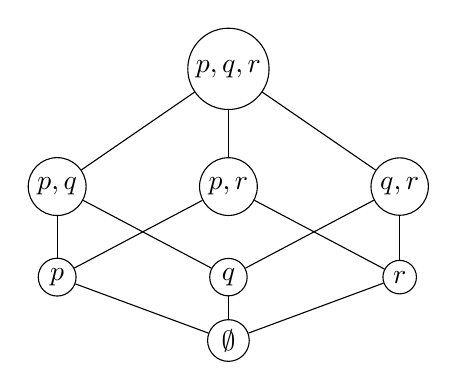
\begin{tikzpicture}[
        setnode/.style={draw,circle,inner sep=2pt},
        every edge/.style={draw},
        x=1.45cm,y=1.15cm
      ]
      \node[setnode] (empty) at (0,0) {\(\emptyset\)};

      \node[setnode] (p) at (-1.5,0.7) {\(\set{p}\)};
      \node[setnode] (q) at (0,0.7) {\(\set{q}\)};
      \node[setnode] (r) at (1.5,0.7) {\(\set{r}\)};

      \node[setnode] (pq) at (-1.5,1.7) {\(\set{p,q}\)};
      \node[setnode] (pr) at (0,1.7) {\(\set{p,r}\)};
      \node[setnode] (qr) at (1.5,1.7) {\(\set{q,r}\)};

      \node[setnode] (pqr) at (0,3) {\(\set{p,q,r}\)};

      \path
        (empty) edge (p)
        (empty) edge (q)
        (empty) edge (r)
        (p) edge (pq)
        (p) edge (pr)
        (q) edge (pq)
        (q) edge (qr)
        (r) edge (pr)
        (r) edge (qr)
        (pq) edge (pqr)
        (pr) edge (pqr)
        (qr) edge (pqr);
    \end{tikzpicture}
    \caption{Diagramma di Hasse del reticolo \(\langle 2^{\{p,q,r\}},\subseteq\rangle\).}
    \label{fig:ctl-power-set-lattice}
  \end{figure}

  Il nodo inferiore rappresenta \(\bot=\emptyset\), quello superiore rappresenta \(\top=W\). L'estremo superiore di due nodi è la loro unione, mentre l'estremo inferiore è la loro intersezione.
\end{example}

\begin{definition}{Funzioni monotone}
  Una funzione \(f: P \to P\) su un ordine parziale è \keyword{monotona} se \(\forall p_1, p_2 \in P\), \(p_1 \sqsubseteq p_2 \implies f(p_1) \sqsubseteq f(p_2)\); è \keyword{anti-monotona} se \(p_1 \sqsubseteq p_2 \implies f(p_2) \sqsubseteq f(p_1)\).
\end{definition}

\subsection{I teoremi di Tarski e Kleene}

\begin{theorem}{Tarski}
  Sia \(f: P \to P\) monotona su un ordine parziale completo. Allora il minimo punto fisso \(\mu x . f(x)\) e il massimo punto fisso \(\nu x . f(x)\) di \(f\) esistono, sono unici, e valgono:
  \[\mu x . f(x) = \bigsqcap \set{x\in P}[f(x) \sqsubseteq x] \qquad \nu x . f(x) = \bigsqcup \set{x\in P}[x \sqsubseteq f(x)]\]
\end{theorem}

Il teorema di Tarski garantisce esistenza e unicità, ma la caratterizzazione non è direttamente computazionale. Kleene fornì una caratterizzazione iterativa: definendo le iterate di \(f\) come
\[f^k(x) = \begin{cases}
    x             & ,k = 0 \\
    f(f^{k-1}(x)) & ,k > 0
  \end{cases}\]

\begin{theorem}{Kleene}
  Per \(f\) monotona e continua su un ordine parziale completo con minimo \(\bot\) e massimo \(\top\):
  \[\mu x . f(x) = \bigsqcup_{k\in\N} f^k(\bot) \qquad \nu x . f(x) = \bigsqcap_{k\in\N} f^k(\top)\]
\end{theorem}

Questa caratterizzazione è computazionalmente utile: se l'ordine ha catene finite (come \(2^W\) con \(W\) finito), l'iterazione si stabilizza in un numero finito di passi, e otteniamo un algoritmo generico:

\begin{algorithmdesc}{Calcolo del minimo punto fisso}
  \begin{algorithmic}[1]
    \Statex{} \textbf{signature} \(\textsc{LFP:} \quad \mathcal{P} \times \mathcal{P}^{\mathcal{P}} \to \mathcal{P} \)
    \Function{\(\textsc{LFP}\)}{$(P,\sqsubseteq,\bot,\top), f$} % chktex 46
    \State{} \(x_0 \gets \bot\)
    \State{} \(x_1 \gets f(x_0)\)
    \State{} \(j \gets 1\)
    \While{\(x_j \neq x_{j-1}\)}
    \State{} \(x_{j+1} \gets f(x_j)\) \Comment{\(x_j = f^j(\bot)\)}
    \State{} \(j \gets j + 1\)
    \EndWhile{}
    \State{} \Return{} \(x_j\)
    \EndFunction{}
  \end{algorithmic}
\end{algorithmdesc}

Per il massimo punto fisso (\textsc{GFP}) l'algoritmo è identico, con l'inizializzazione \(x_0 \gets \top\).

\section{Model checking di \(CTL\) come punto fisso}

Applichiamo ora la teoria al nostro contesto. Definiamo la \keyword{denotazione} di una formula \(\phi\) come l'insieme degli stati che la soddisfano:
\[\den{\phi}[][K] = \set{w \in W}[K,w\models \phi]\]

Si può notare che \(\phi_1 \to \phi_2 \implies \den{\phi_1} \subseteq \den{\phi_2}\). Astraendo il one-step unfolding di \(EU\) in una funzione su insiemi di stati:

\[f_U (V) = \den{\phi_2 \lor (\phi_1 \land EX\, V)} = \den{\phi_2} \cup \left(\den{\phi_1}\cap pre(V)\right) \]

dove \(pre(V) = \den{EX\, V}\) è la \keyword{preimmagine} di \(V\):
\[pre(V) = \set{w \in W}[\exists v \in V\st (w,v) \in R]\]

Dualmente per \(EG\):
\[f_G (V) = \den{\phi} \cap pre(V)\]

\begin{proposition}{Monotonia di \(pre\), \(f_U\) e \(f_G\)}
  \(V_1 \subseteq V_2 \implies pre(V_1)\subseteq pre(V_2)\), e di conseguenza \(f_U\) e \(f_G\) sono monotone su \(\langle 2^W, \subseteq\rangle\).
\end{proposition}
\begin{proof}
  Sia \(w \in pre(V_1)\): allora esiste \(v \in V_1\) con \((w,v) \in R\); ma \(V_1 \subseteq V_2\) implica \(v \in V_2\), e dunque \(w \in pre(V_2)\).
  Per \(f_U\) e \(f_G\): intersezioni e unioni con insiemi costanti rispetto a \(V\) preservano l'inclusione, poiché \(V_1 \subseteq V_2\) implica \(W'\cap V_1 \subseteq W'\cap V_2\) e \(W'\cup V_1 \subseteq W'\cup V_2\) per ogni \(W'\) costante.
\end{proof}

Per il teorema di Kleene possiamo dunque calcolare minimi e massimi punti fissi di \(f_U\) e \(f_G\). Resta da dimostrare che questi coincidano effettivamente con le denotazioni degli operatori \(CTL\)\@.

\begin{theorem}{Caratterizzazione a punto fisso di \(EU\) e \(EG\)}
  \[\den{E (\phi_1 U \phi_2)} = \mu V . f_U(V) \qquad \den{EG \phi} = \nu V . f_G(V)\]
\end{theorem}
\begin{proof}
  Dal one-step unfolding segue immediatamente che \(\den{E (\phi_1 U \phi_2)}\) e \(\den{EG\phi}\) sono punti fissi rispettivamente di \(f_U\) e \(f_G\): dunque \(\mu V . f_U(V)\subseteq \den{E (\phi_1 U \phi_2)}\) (il minimo punto fisso è incluso in ogni punto fisso) e \(\den{EG \phi} \subseteq \nu V. f_G(V)\) (Il massimo punto fisso include ogni punto fisso). Dobbiamo mostrare le inclusioni rimanenti.

  \begin{description}
    \item[\(\den{E (\phi_1 U \phi_2)} \subseteq \mu V . f_U(V)\).] 
    Essendo \(\mu V.f_U(V)\) un punto fisso, vale \(\den{\phi_2} \cup \left(\den{\phi_1}\cap pre(\mu V . f_U(V))\right) = \mu V . f_U(V)\), e in particolare \(\den{\phi_2} \subseteq \mu V . f_U(V)\).
    Procediamo per induzione sulla posizione \(i\) del primo punto che soddisfa \(\phi_2\) lungo un percorso testimone. Sia \(\hat{w} \in \den{E(\phi_1 U \phi_2)}\) e \(\hat{\pi} \in Path(K,\hat{w})\) un percorso con \(\hat\pi \models \phi_1 U \phi_2\) il cui primo punto che soddisfa \(\phi_2\) è \(i\).
    Per \(i = 0\), \(\hat{w} = {(\hat{\pi})}_0 \in \den{\phi_2} \subseteq \mu V . f_U(V)\).
    Per \(i > 0\), scriviamo \(\hat{\pi} = \hat{w}\, \pi\), dove \(\pi\) soddisfa \(\phi_1 U \phi_2\) con primo testimone in posizione \(i - 1\). Detto \(w = {(\pi)}_0\), per ipotesi induttiva \(w \in \mu V . f_U(V)\), e per definizione di \(pre\) si ha \(\hat{w} \in pre(\mu V . f_U(V))\). Inoltre \(\hat{w}\) non soddisfa \(\phi_2\) (per minimalità di \(i\)), dunque deve soddisfare \(\phi_1\), ovvero \(\hat{w}\in \den{\phi_1}\). Quindi
    \[\hat{w}\in \den{\phi_1}\cap pre(\mu V . f_U(V))\subseteq \den{\phi_2}\cup \left(\den{\phi_1}\cap pre(\mu V . f_U(V))\right) = \mu V . f_U(V)\]
    
    \item{\(\nu V . f_G(V) \subseteq \den{EG \phi}\).}
    Essendo \(\nu V . f_G(V)\) un punto fisso, vale \(\nu V . f_G(V) = \den{\phi} \cap pre(\nu V . f_G(V))\). Sia \(w \in \nu V . f_G(V)\): allora \(w \in \den{\phi}\) e \(w \in pre(\nu V . f_G(V))\), ovvero \(w\) ha almeno un successore ancora nel punto fisso. Iterando, da \(w\) si costruisce un percorso infinito che rimane dentro \(\nu V . f_G(V) \subseteq \den{\phi}\): tale percorso testimonia \(EG\phi\). Formalmente, supponendo per assurdo che ogni percorso da \(w\) raggiunga uno stato in cui \(\phi\) non è soddisfatta, per induzione sulla lunghezza del minimo prefisso che porta a tale stato si mostra che \(w \notin \nu V . f_G(V)\), assurdo.
  \end{description}
\end{proof}

\subsection{Algoritmi a punto fisso}

L'algoritmo per \(EU\) ed \(EG\) è dunque un'istanza di \textsc{LFP}/\textsc{GFP} con \(f = f_U\) (partendo da \(V_0 = \emptyset\)) o \(f = f_G\) (partendo da \(V_0 = W\)). Espandendo \(f_U\), la versione estesa per \(EU\) è:

\begin{algorithmdesc}{Compute \(EU\) come minimo punto fisso}
  \begin{algorithmic}[1]
    \Statex{} \textbf{signature} \(\textsc{ComputeEU:} \quad Kripke \times Formula \times Formula \to 2^W \)
    \Function{\(\textsc{ComputeEU}\)}{$(K, \phi_1, \phi_2)$} % chktex 46
    \State{} \(v_0 \gets \emptyset\) \Comment{\(\den{\bot}\)}
    \State{} \(v_1 \gets \den{\phi_2}\)
    \State{} \(j \gets 1\)
    \While{\(v_j \neq v_{j-1}\)}
    \State{} \(j \gets j + 1\)
    \State{} \(T \gets v_{j-1}\)
    \State{} \(V\gets \emptyset\)
    \While{\(T \neq \emptyset\)} \Comment{calcolo di \(pre(v_{j-1})\)}
    \State{} \(s \gets\) choose \(T\)
    \State{} \(T \gets T\setminus\set{s}\)
    \For{\(t \in R^{-1}(s)\)}
    \State{} \(V \gets V\cup\set{t}\)
    \EndFor{}
    \EndWhile{}
    \State{} \(v_{j} \gets \den{\phi_2} \cup \left(\den{\phi_1} \cap V\right)\)
    \EndWhile{}
    \State{} \textbf{return} \(v_j\)
    \EndFunction{}
  \end{algorithmic}
\end{algorithmdesc}

\begin{note}{}
  La formulazione a punto fisso può sembrare solo una rilettura elegante degli algoritmi di etichettatura, ma è molto di più: il calcolo iterato di \(pre\), unioni e intersezioni su insiemi di stati è esattamente ciò che sapremo implementare in modo \emph{simbolico} tramite OBDD, senza mai enumerare esplicitamente gli stati. Questo sarà l'argomento del prossimo capitolo.
\end{note}

\section{Model checking di \texorpdfstring{\(CTL^*\)}{CTL*}}

Torniamo ora alla logica completa \(CTL^*\) e vediamo come risolverne il model checking combinando le tecniche di LTL e \(CTL\)\@.

Consideriamo la proprietà \(E F(p\land X q)\): non è una formula \(CTL\) (l'operatore \(X\) non è preceduto da un quantificatore), ma è della forma \(Q\, \psi\) con \(Q\) quantificatore e \(\psi\) formula LTL\@. In questi casi bastano gli strumenti della~\Cref{sec:buchi}: per \(E\psi\) è sufficiente intersecare l'automa della struttura di Kripke con \(A_\psi\) e verificare che il linguaggio sia non vuoto; per \(A\psi\), dualmente, si verifica che l'intersezione con \(A_{\neg\psi}\) sia vuota:
\[K,w\models Q\psi \iff \begin{cases}
    \mathcal{L}(A_{\psi} \Cap A_{K,w}) \neq \emptyset       & ,Q = E \\
    \mathcal{L}(A_{\neg \psi} \Cap A_{K,w}) = \emptyset & ,Q = A
  \end{cases}\]

Consideriamo però \(E(X (E \psi) \land G (A \psi'))\), che non è né LTL quantificata né \(CTL\)\@. L'idea dell'etichettatura bottom-up torna utile: da grammatica, i casi base di ogni formula \(CTL^*\) sono formule LTL quantificate, che sappiamo risolvere. Una volta etichettati gli stati con una sottoformula quantificata \(Q\psi\), possiamo considerarla come una \emph{nuova proposizione atomica} \(p_{Q\psi}\), sostituirla nella formula esterna, e procedere ricorsivamente: a ogni passo la formula più interna torna a essere della forma \(Q\, \psi_{LTL}\), riapplicando il caso base.

\begin{example}{}
  Prendiamo \(\phi \equiv EX(EG(EFp)) \land G(AF(p\land X(EXq)))\). L'albero di dipendenze tra sottoformule quantificate, derivato dall'albero sintattico, è:

  \begin{center}
    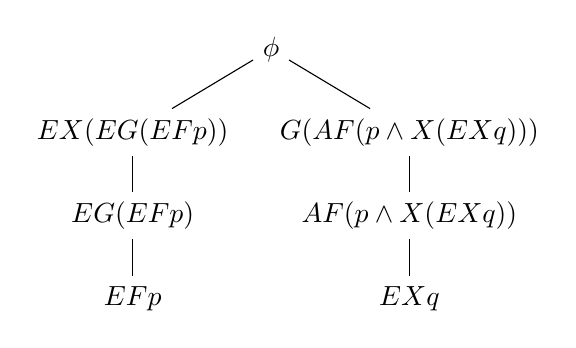
\begin{tikzpicture}[sibling distance=10em, level distance=3em]
      \node {\(\phi\)}
      child { node {\(EX(EG(EFp))\)}
          child { node {\(EG(EFp)\)}
              child { node {\(EFp\)}}
            }
        }
      child { node {\(G(AF(p\land X(EXq)))\)}
          child { node {\(AF(p\land X(EXq))\)}
              child { node {\(EXq\)}}
            }
        };
    \end{tikzpicture}
  \end{center}

  Il flattening con le proposizioni atomiche fresche procede dalle foglie verso la radice:

  \begin{center}
    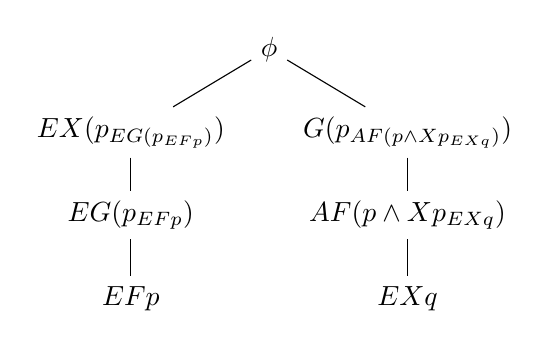
\begin{tikzpicture}[sibling distance=10em, level distance=3em]
      \node {\(\phi\)}
      child { node {\(EX(p_{EG(p_{EFp})})\)}
          child { node {\(EG(p_{EFp})\)}
              child { node {\(EFp\)}}
            }
        }
      child { node {\(G(p_{AF(p\land X p_{EXq})})\)}
          child { node {\(AF(p\land X p_{EXq})\)}
              child { node {\(EXq\)}}
            }
        };
    \end{tikzpicture}
  \end{center}
\end{example}

La complessità di questo algoritmo è \(n\) volte quella del model checking LTL (PSPACE), con \(n\) numero di sottoformule quantificate, lineare nella lunghezza della formula: la complessità totale resta dunque PSPACE\@. Un approccio alternativo usa gli automi ad albero, ottenendo anch'esso PSPACE\@. Per soddisfacibilità e validità, invece, si può mostrare che \(CTL^*\) arriva a 2EXPTIME, a differenza di LTL che rimane PSPACE\@.

\section{Espressività a confronto: LTL, \(CTL\) e \texorpdfstring{\(CTL^*\)}{CTL*}}

\(CTL^*\) offre un notevole guadagno di espressività. LTL è contenuta in \(CTL^*\), poiché ogni formula \(\psi \in LTL\) equivale ad \(A \psi\) in \(CTL^*\). È interessante anche il problema inverso: data \(\phi \in CTL^*\), esiste \(\psi \in LTL\) tale che \(\phi \equiv A\psi\)?

È stato dimostrato che, presa una formula in \(CTL^*\) ed eliminando semplicemente tutti i quantificatori di percorso, si ottiene una formula LTL che è \emph{l'unica candidata possibile}: se esiste una formula LTL equivalente all'originale (una volta quantificata universalmente), è quella. Di conseguenza, data \(\phi \in CTL^*\), si produce \(\hat{\phi} \in LTL\) eliminando i quantificatori e si verifica se \(\phi \equiv A \hat{\phi}\), riducendo il problema alla soddisfacibilità della formula \(\neg ((\phi \to A \hat{\phi}) \land (A\hat{\phi} \to \phi))\): se è soddisfacibile le formule non sono equivalenti, altrimenti lo sono. Essendo \(CTL\) un frammento di \(CTL^*\), lo stesso procedimento si applica anche a formule \(CTL\)\@.

La domanda inversa, ovvero se data \(\psi \in LTL\) esista \(\phi \in CTL\) tale che \(A\psi \equiv \phi\), è invece decidibile caso per caso ma la caratterizzazione generale è a oggi un problema aperto.

\subsection{Formule \texorpdfstring{\(CTL^*\)}{CTL*} non esprimibili in \(CTL\)}

\begin{example}{\(A FGp\)}
  Consideriamo il modello con tre stati: uno stato \(p\) con self-loop, da cui si passa a uno stato \(\neg p\), da cui si passa a un secondo stato \(p\) con self-loop.
  La struttura e la sua estensione ad albero sono mostrate in figura. Nel modello, il primo stato \(p\) ha due possibilità: rimanere in sé stesso oppure passare allo stato \(\neg p\). Dallo stato \(\neg p\) si raggiunge necessariamente il secondo stato \(p\), che ha poi un self-loop.

  \begin{figure}[H]
    \centering
    \begin{tikzpicture}[shorten >=1pt,node distance=1.35cm,on grid,auto,font=\small]
      
      \node[state] (af_s0) {\(s_0\)};
      \node[state] (af_s1) [right=of af_s0] {\(s_1\)};
      \node[state] (af_s2) [right=of af_s1] {\(s_2\)};
      \path[->]
        (af_s0) edge [loop above] ( )
        (af_s0) edge (af_s1)
        (af_s1) edge (af_s2)
        (af_s2) edge [loop above] ( );
      \node[below=0.3cm of af_s0] {\(p\)};
      \node[below=0.3cm of af_s1] {\(\neg p\)};
      \node[below=0.3cm of af_s2] {\(p\)};
            \end{tikzpicture}
    \caption{Il modello per \(A FGp\)}\label{fig:ctl-afgp-model}
  \end{figure}

  In questo modello vale \(A FGp\): ogni percorso da un certo punto in poi rimane per sempre in uno stato \(p\). Proviamo a tradurla in \(CTL\)\@. Le candidate più ovvie sono \(AF(AGp)\) e \(AF(EGp)\). La prima è già falsa nel modello di esempio: nel percorso che rimane per sempre nel primo stato \(p\), nessuno stato soddisfa \(AGp\), perché da ogni prefisso è sempre possibile deviare verso \(\neg p\). La seconda è vera nel modello dato, ma esistono altri modelli in cui \(AFGp\) è vera e \(AF(EGp)\) no, poiché la prima formula richiede che ogni percorso \textit{prima o poi} soddisfi \textit{sempre} \(p\), mentre la seconda richiede che ogni percorso \textit{prima o poi} abbia un \textit{sottopercorso} in cui \(p\) è sempre vero. Una possibile lettura del problema è che la natura esistenziale del testimone di \(F\) mal si combina con la quantificazione universale esterna.
\newline
  Consideriamo ora la formula \(AF(p \land Xp)\).
  La candidata ovvia \(AF(p \land AXp)\) è falsa già nel modello dell'esempio precedente: nel percorso di soli \(p\), ogni stato ha almeno un successore etichettato \(\neg p\), mentre \(AF(p \land Xp)\) è vera. Considerando invece \(AF (p\land EXp)\), questa è soddisfatta dal modello seguente:

  \begin{figure}[H]
    \centering
    \begin{tikzpicture}[shorten >=1pt,node distance=1.35cm,on grid,auto,font=\small]
      
      \node[state] (af_s0) {\(s_0\)};
      \node[state] (af_s1) [right=of af_s0] {\(s_1\)};
      \node[state] (af_s2) [right=of af_s1] {\(s_2\)};
      \path[->]
        (af_s1) edge [loop above] ( )
        (af_s0) edge (af_s1)
        (af_s1) edge (af_s2)
        (af_s2) edge [loop above] ( );
      \node[below=0.3cm of af_s0] {\(\neg p\)};
      \node[below=0.3cm of af_s1] {\(p\)};
      \node[below=0.3cm of af_s2] {\(\neg p\)};
            \end{tikzpicture}
    \caption{Il modello per \(A FGp\)}\label{fig:ctl-afgp-model-2}
  \end{figure}
   
   la cui estensione ad albero contiene percorsi in cui non ci sono mai due \(p\) consecutive: la formula originale non è soddisfatta, e dunque le due non sono equivalenti.
\newline
  Infine, considerando una tipica formula per esprimere la Fairness: \(A(GFp\to Fq)\).
  La candidata \(AG(AF p) \to AFq\) sposta lo scope del quantificatore iniziale: modelli che falsificherebbero l'originale possono soddisfare la seconda semplicemente falsificando la premessa dell'implicazione. Le proprietà di fairness sono l'esempio classico di formule \(CTL^*\)/LTL non esprimibili in \(CTL\)\@.
\end{example}

\subsection{Formule \(CTL\) non esprimibili in LTL}

\begin{example}{\(AG(EFp)\)}
  Vogliamo mostrare che non esiste \(\psi \in LTL\) tale che \(AG(EFp) \equiv A\psi\). Supponiamo per assurdo che esista.

  Consideriamo il modello \(K\) mostrato in figura.

  \begin{figure}[H]
    \centering
    \begin{tikzpicture}[shorten >=1pt,node distance=1.55cm,on grid,auto,font=\small]
      \node[state] (ag_s0) {\(s_0\)};
      \node[state] (ag_s1) [right=of ag_s0] {\(s_1\)};
      \node[state] (ag_s2) [above right=of ag_s1] {\(s_2\)};
      \node[state] (ag_s3) [below right=of ag_s1] {\(s_3\)};
      \path[->]
        (ag_s0) edge (ag_s1)
        (ag_s1) edge (ag_s2)
        (ag_s1) edge (ag_s3)
        (ag_s2) edge [loop above] ()
        (ag_s3) edge [loop below] ();
      \node[below=0.3cm of ag_s0] {\(\neg p\)};
      \node[below=0.3cm of ag_s1] {\(\neg p\)};
      \node[below=0.3cm of ag_s2] {\(\neg p\)};
      \node[below=0.3cm of ag_s3] {\(p\)};
    \end{tikzpicture}
    \caption{Il modello \(K\) per la dimostrazione di \(AG(EFp)\).}\label{fig:ctl-agefp-model}
  \end{figure}
   
   Poiché \(s_3\) è raggiungibile da \(s_0\), \(K \models AG(EFp)\), e dunque \(K \models A\psi\).

  Consideriamo ora il modello \(K'\) ottenuto rimuovendo \(s_3\): qui \(p\) non è mai soddisfatta, dunque \(K' \not\models AG(EFp)\). Ma tutti i percorsi infiniti di \(K'\) sono anche percorsi di \(K\): essendo che le formule LTL sono valutate sui percorsi, da \(K \models A\psi\) segue \(K' \models A\psi\), e quindi \(K' \models AG(EFp)\), assurdo.
\end{example}

\subsection{La gerarchia di espressività}

Riassumendo, LTL (intesa come frammento delle \(A\psi\)) e \(CTL\) sono incomparabili, entrambe strettamente contenute in \(CTL^*\):
\begin{itemize}
  \item \(A (p U q)\) appartiene all'intersezione di LTL e \(CTL\);
  \item \(AG(EFp)\) è esprimibile solo in \(CTL\);
  \item \(AF(p \land Xp)\) e \(A(GFp \to Fq)\) sono esprimibili solo in LTL;
  \item la congiunzione di una formula solo-CTL e una solo-LTL è esprimibile solo in \(CTL^*\).
\end{itemize}
\begin{figure}[H]
  \centering
  \begin{tikzpicture}[
      set/.style={draw, thick, ellipse, minimum width=5.3cm, minimum height=3.9cm,
        align=center},
      example/.style={font=\scriptsize, align=center}
    ]
    \node[draw, thick, fill=none, minimum width=14cm, minimum height=8cm,
      rounded corners=2pt] (frame) {};
    \node[set, fill=green!18, minimum width=11.2cm, minimum height=6.5cm] (ctls) {};
    \node[above=0.1cm of ctls.north, text=green!50!black] {\(CTL^*\)};
    \node[set, fill=blue!18, fill opacity=0.72, text opacity=1,
      xshift=-1.45cm] (ltl) {};
    \node[above=0.1cm of ltl.north, text=blue!60!black] {\(LTL\)};
    \node[set, fill=orange!25, fill opacity=0.72, text opacity=1,
      xshift=1.45cm] (ctl) {};
    \node[above=0.1cm of ctl.north, text=orange!80!black] {\(CTL\)};

    \node[example, below left=0.25cm and 0.05cm of ltl.center]
      {$A(GFp\to Fq)$};
    \node[example, below right=0.25cm and 0.05cm of ctl.center]
      {$AG(EFp)$};
    \node[example, above=2.5cm of ctls.south]
      {$A(p\,U\,q)$};
    \node[example, below=0.25cm of ctls.south]
      {CTL e LTL incomparabili};
  \end{tikzpicture}
  \caption{Gerarchia di espressività tra LTL, CTL e \(CTL^*\).}\label{fig:ctl-expressiveness-hierarchy}
\end{figure}